\documentclass[bwprint, withoutpreface]{cumcmthesis}

\usepackage{extarrows}
\usepackage{authblk}
\usepackage{tikz}
\usetikzlibrary{intersections}

\title{实变第二章总结}

\begin{document}
\maketitle
\noindent Author: Tony Xiang

\noindent Full Document can be acquired here: 

\noindent https://github.com/T0nyX1ang/RealAnaly-Documents/blob/master/Chapter\%202/Chapter2.pdf

\noindent Full Source code can be downloaded here:

\noindent https://github.com/T0nyX1ang/RealAnaly-Documents/blob/master/Chapter\%202/Chapter2.tex

\section{引言}
\indent 测度的四条性质:\textbf{非负性,可列可加性,平移不变性,可减性}.

区间的长度:
\begin{equation*}
	|I| = 
	\begin{cases}
		b - a, \quad \mbox{$I$为有界区间}, I = (a, b), (a, b], [a, b), [a, b] \\
		+\infty, \quad \mbox{$I$为无界区间}
	\end{cases}	
\end{equation*}

方体的体积:$I = I_1 \times I_2 \times \cdots I_n$,则体积为:$|I| = |I_1| \times |I_2| \times \cdots |I_n|$.

只要有一个区间是无界的,整个方体即为无界方体,其体积为$+\infty$.另外有$|\emptyset| = 0$.

规定:$a + (+\infty) = (+\infty) + a = +\infty$,$(+\infty) + (+\infty) = +\infty$.

\section{外测度}
\indent 开方体覆盖.

\textbf{外测度:}对每个$A \subset \mathbb{R}^n$,令
\begin{equation*}
	m^*(A) = \inf{\sum_{k = 1}^{\infty}\{{I_k}: \{I_k\} \mbox{是$A$的开方体覆盖}\}}.
\end{equation*}
称$m^*(A)$为$A$的Lebesgue外测度.

注意:$\forall A \subset \mathbb{R}^n$,$m^*(A) \geqslant 0$(非负性).若对$A$的任一开方体覆盖$\{I_k\}$,有$\sum_{k = 1}^{\infty}|I_k| = \infty$,则$m^*(A) = \infty$.即$0 \leqslant m^*(A) \leqslant \infty$.

回顾下确界的定义:$a = \inf E$,则
\begin{itemize}[itemindent=2em]
	\item $\forall x \in E, a \leqslant x$.
	\item $\forall \varepsilon > 0, \exists x' \in E, s.t. \quad x' < a + \varepsilon$.
\end{itemize}

由此得出外测度的两个事实:
\begin{itemize}[itemindent=2em]
	\item \textbf{事实1:} $\forall {I_k} \supset A, s.t. \quad m^*(A) \leqslant \sum_{k = 1}^{\infty}|I_k|$.
	\item \textbf{事实2:} $m^*(A) < \infty, \forall \varepsilon > 0, \exists {I_k} \supset A, s.t. \quad \sum_{k = 1}^{\infty}|I_k| < m^*(A) + \varepsilon$.
\end{itemize}

注意:事实2可以由$\varepsilon$的任意性进行改进,如$\varepsilon \to \frac{\varepsilon}{2^k}$,这是为了无限求和之后仍可保持$\varepsilon$.

\textbf{一个重要的数分定理:设$a, b \in \mathbb{R}^1, \forall \varepsilon > 0, s.t. \quad a < b + \varepsilon$,则$a \leqslant b$.}

外测度的性质:
\begin{itemize}[itemindent=2em]
	\item 可数集的外测度为$0$.(用$I_k = (a_k - \frac{\varepsilon}{2^{k + 1}}, a_k + \frac{\varepsilon}{2^{k + 1}})$覆盖$A$.)
	\item $m^*(\emptyset) = 0$.
	\item 单调性:$A \subset B \Rightarrow m^*(A) \leqslant m^*(B)$. (由事实1,2与数分定理可得.)
	\item \textbf{次可列可加性:}对$\mathbb{R}^n$中的任意一列集$\{I_k\}$,有:
	\begin{equation*}
		m^*(\bigcup_{k = 1}^{\infty}{I_k}) \leqslant \sum_{k = 1}^{\infty}{m^*(I_k)}.
	\end{equation*}(将事实2进行改进:$\sum_{i = 1}^{\infty}|I_{k, i}| \leqslant m^*(A_k) + \frac{\varepsilon}{2^k}$,之后再二重求和即可.)
	\item \textbf{次有限可加性:}对$\mathbb{R}^n$中的任意一列集$\{I_k\}$,有:
	\begin{equation*}
		m^*(\bigcup_{k = 1}^{n}{I_k}) \leqslant \sum_{k = 1}^{n}{m^*(I_k)}.
	\end{equation*}(次可列可加性的推论.)
	\item 平移不变性:$E \subset \mathbb{R}^n, \forall x_0 \in \mathbb{R}^n, m^*(x_0 + E) = m^*(E)$,$x_0 + E = \{x_0 + x: x \in E\}.$ (由事实1,2与对偶的性质证明.)
	\item 数乘的性质:$E \subset \mathbb{R}^n, \forall \lambda \in \mathbb{R}, m^*(\lambda E) = |\lambda|^n m^*(E)$,$\lambda E = \{\lambda x: x \in E\}.$ (由事实1,2与对偶的性质证明.)
\end{itemize}

注意:次可列可加性是外测度中“不太好”的性质,它没有集合不相交的条件限制.

$m^*(I) = |I|$,$I$为$\mathbb{R}^n$中方体.这是外测度与体积的对应.(分区间是有限的与区间是无限的两个部分证明,有限部分利用事实2,有限覆盖定理,外测度的单调性与夹逼定理证明,无限部分取任意大的数$k$,都有$[a, a + k] \subset [a, +\infty]$,$k \leqslant m^*([a, +\infty])$.)

注意:有限覆盖定理指:一族开区间覆盖一个区间$I$,则必能找到有限的区间,将区间$I$覆盖.

\section{可测集与测度}
\subsection{定义与性质}

\indent $m^*(A) = m^*(A \cap E) + m^*(A \cap E^C) \Leftrightarrow m^*(I) = m^*(I \cap E) + m^*(I \cap E^C)$

\textbf{Caratheodory条件:}$m^*(A) = m^*(A \cap E) + m^*(A \cap E^C)$.

\begin{center}
	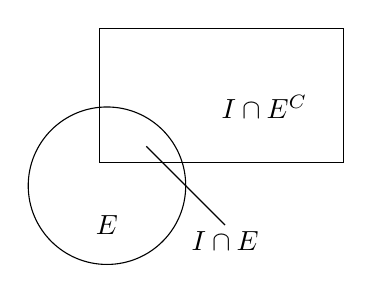
\begin{tikzpicture}
	\draw (0, 0) circle [radius=1cm];
	\draw (-0.1, 0.3) rectangle (3, 2);
	\draw (0, -0.5) node {$E$};
	\draw (0.5, 0.5) -- (1.5, -0.5);
	\draw (1.5, -0.7)node {$I \cap E$};
	\draw (2, 1) node {$I \cap E^C$};
\end{tikzpicture} \qquad
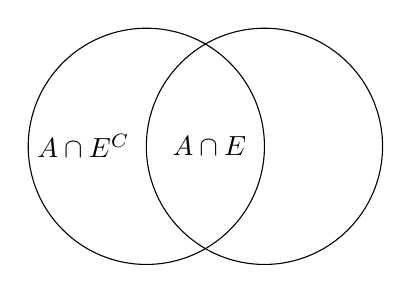
\begin{tikzpicture}
	\draw (0, 0) circle [radius=1.5cm];
	\draw (1.5, 0) circle [radius=1.5cm];
	\draw (-0.8, 0) node {$A \cap E^C$};
	\draw (0.8, 0) node {$A \cap E$};
\end{tikzpicture}
\end{center}

\textbf{可测集:}$E \subset \mathbb{R}^n, \forall A \subset \mathbb{R}^n$,Caratheodory条件成立,称$E$为Lebesgue可测集.

\textbf{可测集的测度:}若$E$为Lebesgue可测集,则称$m^*(E)$为$E$的Lebesgue测度,记为$m(E)$.

Caratheodory条件等价于$m^*(A) \geqslant m^*(A \cap E) + m^*(A \cap E^C)$成立.

\textbf{外测度为零的集合是可测集,称其为零测集.}

\textbf{零测集的子集为可测集.}

\textbf{可数集是可测集,且测度为零,特别地,$m(\mathbb{Q}) =0$.}

$\mathbb{R}^n$中的每个方体是可测集,且其测度等于方体的体积.(用Caratheodory条件,$J \cap {I^C} = \bigcap_{i = 1}^{k}{I_i}$,且这些集合互不相交.)

\textbf{可测集的性质:}
\begin{itemize}[itemindent=2em]
	\item 若$E_1, E_2, \cdots, E_n$为可测集,则$\bigcup_{i = 1}^{k}{E_k}$为可测集.
	证明在$k = 2$时成立,$E = E_1 \cup E_2$,$E = E_1 \cup (E_2 - E_1) = E_1 \cup ({E_1}^C \cap E_2)$.
	\item 若$E_1, E_2, \cdots, E_n$为互不相交的可测集,$A_i \subset E_i$,则$m^*(\bigcup_{i = 1}^{k}{A_i}) = \sum_{i = 1}^{k}{m^*(A_i)}$.
	证明在$k = 2$时成立,$(A_1 \cup A_2) \cap E_1 = A_1$,$(A_1 \cup A_2) \cap {E_1}^C = A_2$.
\end{itemize}

\begin{center}
	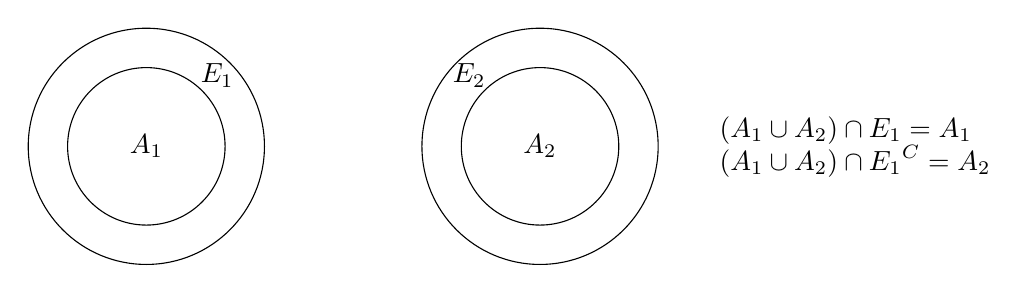
\begin{tikzpicture}
		\draw (0, 0) circle [radius=1cm];
		\draw (0, 0) circle [radius=1.5cm];
		\draw (0, 0) node {$A_1$};
		\draw (0.9, 0.9) node {$E_1$};
		\draw (5, 0) circle [radius=1cm];
		\draw (5, 0) circle [radius=1.5cm];
		\draw (5, 0) node {$A_2$};
		\draw (4.1, 0.9) node {$E_2$};
		\node [below, align=justify] at (9, 0.5) {$(A_1 \cup A_2) \cap E_1 = A_1$ \\ $(A_1 \cup A_2) \cap {E_1}^C = A_2$};
	\end{tikzpicture}		
\end{center}

\begin{itemize}[itemindent=2em]
	\item 可测集的全体是一个$\sigma$-代数.
	首先可测集的全体是一个代数,证明$\mathcal{M}(\mathbb{R}^n)$对不相交可列并封闭,利用上一个性质,Caratheodory条件并进一步取极限即可.
	\item $\mathcal{B}(\mathbb{R}^n) \subset \mathcal{M}(\mathbb{R}^n)$,且包含关系为严格包含.
	利用开集构造定理与Borel集的定义即可.
	\item \textbf{有限可加性:}$A_1, A_2, \cdots, A_n$为互不相交的可测集,则$m(\bigcup_{i = 1}^{k}{A_i}) = \sum_{i = 1}^{k}{m(A_i)}$.(性质2中取$A_i = E_i$)
	\item \textbf{可减性:}$A, B \in \mathcal{M}(\mathbb{R}^n), A \subset B, m(A) < \infty$,则$m(A - B) = m(A) - m(B).$(注意$A$的测度是有限的,$B = A \cup (B - A)$,$A \cap (B - A) = \emptyset$)
	\item \textbf{可列可加性:}$\{A_k\}$为一列互不相交的可测集,则$m(\bigcup_{k = 1}^{\infty}{A_k}) = \sum_{k = 1}^{\infty}{m(A_k)}$.(取极限,用测度的次可列可加性分别得到正向与反向的不等式)
	\item \textbf{下连续性:}$\{A_k\}$为一列单调递增的可测集,则$m(\bigcup_{k = 1}^{\infty}{A_k}) = \lim_{k \to \infty} m(A_k)$.(构造不交并$B_1 = A_1, B_k = A_k - A_{k - 1}$,测度的可列可加性)
	\item \textbf{上连续性:}$\{A_k\}$为一列单调递减的可测集,且$m(A_1) < \infty$,则$m(\bigcup_{k = 1}^{\infty}{A_k}) = \lim_{k \to \infty} m(A_k)$. (令$B_k = A_1 - A_k$转化为下连续性的问题,注意证明时会使用可减性,所以上连续性与下连续性不完全相同)
	\item 平移不变性:$E \subset \mathbb{R}^n, \forall x_0 \in \mathbb{R}^n, m(x_0 + E) = m(E)$,$x_0 + E = \{x_0 + x: x \in E\}$.(平移不变性由外测度可知,主要证明$x_0 + E \in \mathcal{M}(\mathbb{R}^n)$,使用$x_0 + A \cap E = (x_0 + A) \cap (x_0 + E), x_0 + E^C = (x_0 + E)^C$)
\end{itemize}

注意:测度继承了外测度的所有性质,所以需要对次可列可加性与可列可加性进行区分,可列可加性需要集合相交,次可列可加性不需要.

\textbf{证明一个集合是可测的方法:}
\begin{itemize}[itemindent=2em]
	\item Caratheodory条件.
	\item 证明它是一个Borel集.
	\item 利用可测集的运算间接证明.
\end{itemize}

\subsection{可测集的逼近定理}
\indent 可测集可以用开集,闭集逼近,可以用$G_{\delta},F_{\sigma}$型集最佳逼近.

\begin{itemize}[itemindent=2em]
	\item $\forall \varepsilon > 0, \exists \mbox{开集}G \supset E, s.t. \quad m(G - E) < \varepsilon$.
	\item $\forall \varepsilon > 0, \exists \mbox{闭集}F \subset E, s.t. \quad m(E - F) < \varepsilon$.
	\item $\exists G_{\delta} \mbox{型集} G \supset E, s.t. \quad m(G - E) = 0$.
	\item $\exists F_{\sigma} \mbox{型集} F \subset E, s.t. \quad m(E - F) = 0$.
\end{itemize}

逼近定理的证明思路:
\begin{itemize}[itemindent=2em]
	\item 将$m(E)$分有限与无穷两种情况讨论.对于有限情况,利用外测度的事实2,用一列开方体${I_k}$覆盖之,作$G = \bigcup_{k = 1}^{\infty}{I_k}$,由测度可减性可知.
	\item 对于无限情况,先找一列互不相交的可测集$\{A_k\}$,$m(A_k) < \infty$且$\mathbb{R}^n = \bigcup_{k = 1}^{\infty}{A_k}$,令$E_k = E \cap A_k$,则$m(E_k) < \infty$且$E = \bigcup_{k = 1}^{\infty}{E_k}$,这样将\textbf{无限测度转化至有限情况}.取$G_k \supset E_k, s.t.\quad m(G_k - E_k) < \frac{\varepsilon}{2^k}$,取$G = \bigcup_{k = 1}^{\infty}{G_k}$,$G - E \subset \bigcup_{k = 1}^{\infty}\{G_k - E_k\}$.使用测度单调性与次可列可加性即可.
	\item 对于第二条,将闭集转化至开集的情况.$E - F = E \cap F^C = {(E^C)}^C \cap G = G - E^C, F = G^C$.
	\item 对于第三条,利用$\varepsilon \to \frac{1}{k}$的转化,将极限转化为集列$\{G_k\}$,作$G = \bigcap_{k = 1}^{\infty}{G_k}$,取极限即可,这个方法很重要.
	\item 对于第四条,利用$\varepsilon \to \frac{1}{k}$的转化,将极限转化为集列$\{F_k\}$,作$F = \bigcup_{k = 1}^{\infty}{F_k}$,取极限即可.
\end{itemize}

\begin{center}
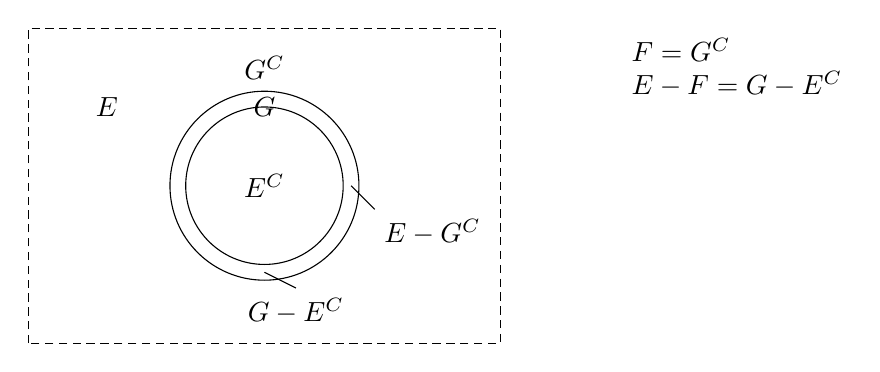
\begin{tikzpicture}
	\draw[densely dashed] (-3, -2) rectangle (3, 2);
	\draw (0, 0) circle [radius=1cm];
	\draw (0, 0) circle [radius=1.2cm];
	\draw (0, 0) node {$E^C$};
	\draw (0, 1) node {$G$};
	\draw (0, -1.1) -- (0.4, -1.3) node[below] {$G - E^C$};
	\draw (-2, 1) node {$E$};
	\draw (0, 1.5) node {$G^C$};
	\draw (1.1, 0) -- (1.4, -0.3) node[below right] {$E - G^C$};
	\node [below, align=justify] at (6, 2) {$F = G^C$ \\ $E - F = G - E^C$};
\end{tikzpicture}
\end{center}

注意:对偶性可以简化很多计算.

注意:每个可测集与一个Borel集仅相差一个零测集,但是这个差距是集合完备与不完备之间的差距.

$[0, 1]$间存在不可测集,可以使用Zermelo选取公理构造.

本节之后的内容不作要求.

\appendix
\section{布置的课后作业}
\indent $1,4,5,6,7,8,9,12,13,15,16,17,18,19,20,21.$

\section{课后作业的讲解}
\indent 4.类似第一章$A$类12题的做法,将直线上的有理开区间转换为$\mathcal{R}^n$中用有理点构成的开方体。仍使用:$A = \bigcup_{x \in A}\{A \cap I_x\}$.

5.$A - B, B - A \in \mathcal{M}(\mathbb{R}^n)$,$B = (A - (A - B)) \cup (B - A)$.

6.$\varepsilon \to \frac{1}{k}$,套路与逼近定理一致.

7.注意如果使用测度的可减性,需要说明测度有限.同时适用于测度公式中的移项操作.

8.测度的下连续性,测度的上连续性.

9.扩展的De Morgan公式可以让我们把全空间设为$[0, 1]$然后作$A$的补集.

12.十进制无限小数的表示,类似Cantor集的构造,十分取其第八区间.

13.利用开集定义,然后作邻域的内接方体.

15.$G = [0, 1] - F$,以是否为空集为条件分情况讨论.

16.$\overline{\mathbb{Q}_0} = [0, 1], \mathbb{Q}_0 = {x \in [0, 1]: x \in \mathbb{Q}^n}$.构造:
\begin{equation*}
	G = (\bigcup_{n = 1}^{\infty}{(r_n - \frac{\varepsilon}{2^{n + 1}}, r_n + \frac{\varepsilon}{2^{n + 1}})}) \cap (0, 1).
\end{equation*}

17.$F = [0, 1] - G$. $G$可以按照上一题方法构造.

18.类似Cantor集构造方法,$a = 1 - c$,然后每次去掉的区间长度相应改变.

\section{一些闲谈}
\indent 注意,以下内容仅代表本人观点。

第二章是对测度论的基本介绍,不涉及抽象测度空间的内容.

有一些有趣的套路,来跟大家分享一下:
\begin{itemize}[itemindent=2em]
	\item 开集与闭集的放缩,即$\varepsilon \to \frac{1}{k}$.这个方法首先转化极小量,然后通过放缩使得开集与闭集进一步逼近目标集合(测度或外测度的单调性),然后极小量趋向无穷,而已经构造好的集合与极小量无关,就将它与目标集合只相差一个零测集.这个方法很巧妙,而且对这类型的题目是通用的,因为开集,闭集,$G_{\delta}$,$F_{\sigma}$型集均可测,性质很好.
	\item 空间的缩小,将全空间缩小至$[0, 1]$上考虑一些问题,注意,求补集是可行的,因为有扩展的De Morgan定理:
	\begin{align*}
		E - \bigcup_{\alpha \in I}{A_{\alpha}} = \bigcap_{\alpha \in I}{E - A_{\alpha}} \\
		E - \bigcap_{\alpha \in I}{A_{\alpha}} = \bigcup_{\alpha \in I}{E - A_{\alpha}}
	\end{align*}
	但是处理开集与闭集时需要小心子集的开闭性质与全空间不完全相同的问题,可能需要通过集合的运算来“打磨”集合.
	\item 可以利用已有的集合构造新的集合,也可以进行一些改造.如Cantor集的变形可以使测度增大.
	\item ...
\end{itemize}

还有一些需要注意的点:
\begin{itemize}[itemindent=2em]
	\item 测度可减性的条件.
	\item 等式的书写,最右边的等号是最后一步的推导结果,最左边的等号是最先推导出的结果,这样可以增强可读性.
\end{itemize}

\end{document}